\documentclass[tikz,border=4pt]{standalone}
\usepackage{tikz}
\usetikzlibrary{arrows.meta,positioning,shapes.geometric}

\begin{document}
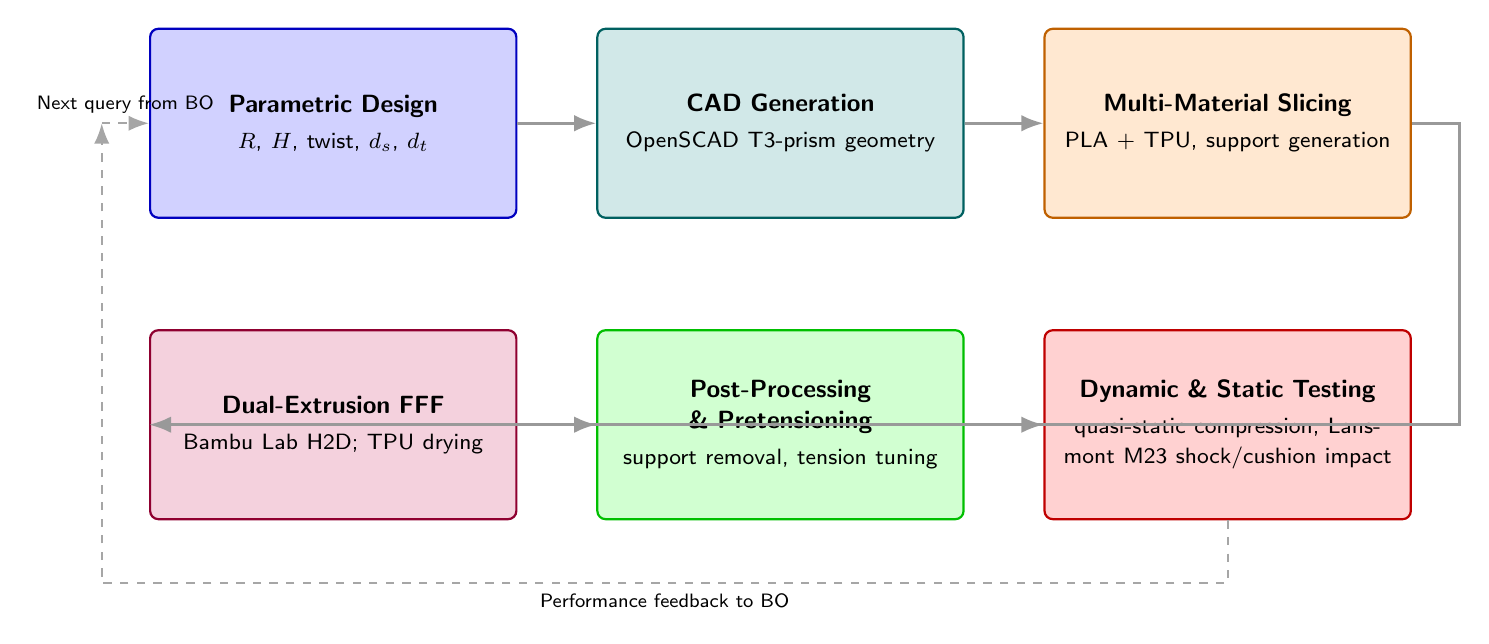
\begin{tikzpicture}[
  font=\sffamily\small,
  node distance=14mm and 10mm,
  stage/.style={
    rectangle,
    rounded corners=3pt,
    draw=#1!75!black,
    fill=#1!18,
    line width=0.8pt,
    minimum height=24mm,
    text width=43mm,
    align=center,
    inner sep=5pt
  },
  arrow/.style={-{Latex[length=2.8mm]}, line width=1.0pt, draw=gray!80},
  looparrow/.style={-{Latex[length=2.6mm]}, dashed, line width=0.8pt, draw=gray!70}
]
  \node[stage=blue] (params) {\textbf{Parametric Design}\\[2pt]
    {\footnotesize $R$, $H$, twist, $d_s$, $d_t$}};
  \node[stage=teal, right=of params] (cad) {\textbf{CAD Generation}\\[2pt]
    {\footnotesize OpenSCAD T3-prism geometry}};
  \node[stage=orange, right=of cad] (slicing) {\textbf{Multi-Material Slicing}\\[2pt]
    {\footnotesize PLA + TPU, support generation}};
  \node[stage=purple, below=of params] (print) {\textbf{Dual-Extrusion FFF}\\[2pt]
    {\footnotesize Bambu Lab H2D; TPU drying}};
  \node[stage=green, right=of print] (post) {\textbf{Post-Processing \& Pretensioning}\\[2pt]
    {\footnotesize support removal, tension tuning}};
  \node[stage=red, right=of post] (testing) {\textbf{Dynamic \& Static Testing}\\[2pt]
    {\footnotesize quasi-static compression; Lansmont M23 shock/cushion impact}};

  \draw[arrow] (params) -- (cad);
  \draw[arrow] (cad) -- (slicing);
  \draw[arrow] (slicing.east) -- ++(6mm,0) |- (print.west);
  \draw[arrow] (print) -- (post);
  \draw[arrow] (post) -- (testing);

  \draw[looparrow] (testing.south) -- ++(0,-8mm) -| node[pos=0.25, below, font=\sffamily\scriptsize]
    {Performance feedback to BO} ([xshift=-6mm]params.west);
  \draw[looparrow] ([xshift=-6mm]params.west) -- node[above, font=\sffamily\scriptsize]
    {Next query from BO} (params.west);
\end{tikzpicture}
\end{document}
